% !TEX TS-program = pdflatex
% !TeX spellcheck = en_US
% !TEX root = main.tex

In this section we present a simplified GUI model which incorporates all important features of the
domain. In the real implementation this simplified model is extended a little bit, but this extension
does not introduce any essential changes into the synthesis algorithm.

We can identify three important aspects of GUI: a \emph{structure}, a \emph{layout}, and a \emph{guideline}.
\emph{Structure} describes the set of GUI controls and their relations; \emph{layout}, on the other hand, determines
their relative placement. This approach aligns well with a common tendency to introduce a separation between business
logic and its visual representation~\cite{UI3}. A \emph{guideline} maps certain controls of a structure into some concrete
layout primitives.

We demonstrate these notions with the following example. Let us have a GUI form shown in Fig.~\ref{form1}. We can describe its structure as follows:

\begin{itemize}
\item there are three GUI controls: a check box, a text label, a drop-down list (combo box);
\item there is a dependency relation between the text label and the combo box since the former \emph{describes} the
  latter; thus, the text label and the combo box constitute a compositional entity;
\item there is an order relation between the checkbox and this compositional entity
  since (as we speculate) there is an implied dependency caused by the importance of the components
  from the perspective of the GUI author.
\end{itemize}

We can depicture this structure as shown in Fig.~\ref{form1-structure-layout}\subref{form1-structure}.
Thus, we can treat a structure as a set of named \emph{relations} between controls (and, possibly, other
data domains such as strings, numbers, etc.). In our approach we divide all such relations into two categories~---
\emph{abstract} and \emph{concrete}. The semantics of \emph{abstract} ones is assigned by a guideline, \emph{concrete}~---
by the system. Concrete relations describe the types of the controls, their various properties (the contents of
text fields, sizes, etc.); they also can be used to combine other controls into ordered or unordered groups or
\emph{virtual controls}~--- containers which incorporate other controls and behave as a whole.

The set of \emph{abstract} relations contains such relations as binary ordering (one control after another), description (one
control contains a description of another, like a label of a check box or text field, etc.), subordination (one control can
be considered as a ``subordinate'' of another, for example, a text field, enabled by a checkbox). But actually these
relations are just conventional abstract names which can be used both in structure descriptions and guidelines. Their
semantics is completely determined by a guideline, and the system does not contain any specific treatment of
these relations. End-users can freely add custom abstract relations and define their semantics in the guidelines.

For a given structure its \emph{layout} can be specified using a set of primitives describing the placement
of controls, their alignment and other similar properties. In the given example the label and combo box are
laid out horizontally next to each other with a certain horizontal inset, the checkbox is stacked over the compositional
label and combo box pair with a certain vertical inset, and the whole layout is left-justified. We can depicture the
layout in question as shown in Fig.~\ref{form1-structure-layout}\subref{form1-layout}. Unlike relations used for
describing structures, all primitives of layout description have a hardcoded semantics which the
synthesis algorithm relies upon.

Finally, a guideline contains a set of rules prescribing what layout primitives should be used for
certain (sub)structures of GUI under certain conditions. In Fig.~\ref{form1-structure-layout}\subref{gdrule}
we show an example of such a rule, taken from \textsc{JetBrains} set of conventional GUI guidelines~\cite{JBG}.
As a rule, GUI guidelines are described in informal terms using a number of examples; in the next section
we present their formal treatment.



\begin{comment}
In our simplified model a structure is completely invariant w.r.t. layout: regardless what a layout could
be the assortment of controls and their logical/functional dependencies remains the same.


We consider connected structures only where each control is related to some other. If the structure can be divided into several
unrelated parts, each of them is laid out independently with possible overlapping.

%Reiterating the example in the Fig.~\ref{form1}, we can now provide a more concrete description of
%its GUI structure (see Fig.~\ref{form1-concrete-structure}).

%From the GUI structure point of view these relations are considered as fully abstract entities. Their semantics
%and impact on the layout is determined by the layout guidelines only.

\subsection{GUI Layout}
\label{constraints}

We have identified the following set of layout primitives:

\begin{itemize}
\item vertical composition of controls (control $C_1$ is laid out directly on the top of the control $C_2$):
  \[
     \term{vert}\,(C_1,\,C_2)
  \]
\item horizontal composition of controls (control $C_1$ is laid out directly to the left of the control $C_2$):
  \[
     \term{hor}\,(C_1,\,C_2)
  \]
\item vertical alignment of controls (does not affect the horizontal position of controls):
  \[
     \term{valign}\,(C_1,\,C_2)
  \]
\item horizontal alignment of controls (does not affect the vertical position of controls):
  \[
     \term{halign}\,(C_1,\,C_2)
  \]
\item horizontal indentation of one control to another:
  \[
  \term{indent}\,(C_1,\,C_2)
  \]
\end{itemize}

%This is a somewhat simplified model; in reality the additional arguments should be specified for these primitives which
%describe the \emph{insets} and \emph{alignments} of the controls being laid out. An inset specifies a desirable vertical
%or horizontal space between controls; as for alignments, different kinds of those are distinguished: top, center, bottom,
%and baseline vertical alignments, and left, right, and center horizontal alignments. As for now we consider the insets
%being a predefined constants and limit the alignments to some default ones; we argue that this choice does not
%undermine the approach we describe.

\begin{figure}[h]
  \centering
  \scalebox{0.8}{
  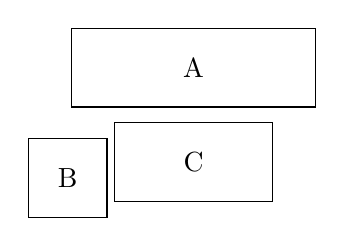
\begin{tikzpicture}
    \node[rectangle,draw,minimum width=3.1cm,minimum height=1cm] (A) at (1.6, 1.4) {A};
    \node[rectangle,draw,minimum width=1cm,minimum height=1cm] (B) at (0,0)        {B};
    \node[rectangle,draw,minimum width=2cm,minimum height=1cm] (C) at (1.6,0.2)    {C};
%    \path[draw,dashed] (1.6, 0.7) -- (4, 0.7);
%    \path[draw,dashed] (1.6, 0.9) -- (4, 0.9);
%    \path[draw] (3.8, 1.3) -- node[above] {\emph{pad}} (3.8, 0.3);
  \end{tikzpicture}}
  \caption{Layout example}
  \label{layout-example}
\end{figure}

This primitives can be independently used for different controls: for example, controls $A$ and $B$ can be composed
vertically, $B$ and $C$~--- horizontally, and $A$ and $C$ can be horizontally aligned by center, which would
provide the following layout (see Fig.~\ref{layout-example}). Note, the constraints in this example do not require
$B$ and $C$ to be aligned \emph{vertically}.
\end{comment}

\FloatBarrier
